\section{Evaluation}
\label{sec:evaluation}
% for LOC run: git ls-files | grep  \.java | xargs wc -l | awk '{ SUM += $1} END { print SUM }'
% for Commits run: bug_column_blame_approach, and then take len(commits) of each project
% for # of contributers (assuming unique), "git checkout --force master" and  "git shortlog -s -n | wc -l"
% for # of commits : git rev-list --count trunk

\subsection{Experiment 1: Ownership and granularity}

\subsubsection{Experiment design}

In this experiment we address research questions 1 and 2 building a model that can classify implicated files using the classic code metrics, and evaluating if the ownership metrics can improve its effectiveness. We also address question 2a comparing the improvement given by different ownership granularities (commit-based and line-based).

\begin{table}[ht]
    \footnotesize
    \centering
    \caption{Class sample size per project}
    \label{tab:sample_size}
    \begin{tabular}{|c|c|c|}
        \hline
        \textbf{Project} & \textbf{Implicated files} & \textbf{Sample size} \\
        \hline
        Camel & 7076 & 4000 \\
        Lucene-Solr & 14416 & 4000 \\
        Mahout & 2114 & 2000 \\
        Maven  & 2383 & 2000 \\
        Zookeeper & 819 & 800 \\
        \hline
    \end{tabular}
\end{table}

This experiment is performed for every considered project using its metrics dataset with the 5\% threshold. We define different subsets of features (see Table~\ref{tab:metric_groups}), and for each one of them we cross-validate (10-folds) the Random Forest~\cite{breiman2001random} model on a sample of the dataset. The sample contains the same number of lines for both the classes (implicated and not implicated, see Table~\ref{tab:sample_size}).


\begin{table}[ht]
    \centering
    \footnotesize
    \caption{Considered set of metrics}
    \label{tab:metric_groups}
    \begin{tabular}{|c|p{0.3\textwidth}|}
        \hline
        \textbf{Group} & \textbf{Metrics} \\
        \hline
        Classic & file\_size, comment\_to\_code\_ratio, previous\_implications \\
        \hline
        Commit based & Classic + commit\_ownership, minor\_contributors, major\_contributors \\
        \hline
        Deleted  & Classic + line\_ownership\_deleted, lines\_deleted\_minor\_contributors, lines\_deleted\_major\_contributors \\
        \hline
        Added  & Classic + line\_ownership\_added, lines\_added\_minor\_contributors, lines\_added\_major\_contributors,\\
        \hline
        Line authorship  & Classic + line\_authorship, total\_authors\\
        \hline
        Line based  & Classic + Added + Deleted \\
        \hline
        All metrics  & All the above mentioned metrics minus the highly correlated ones (cutoff=0.75)\\
        \hline
    \end{tabular}
\end{table}

We evaluate the constructed classifiers with the out-of-bag error rate (OOB) averaged over the 10-folds, and use it to determine if the improvement over the classic metrics is statistically significant. This is done by comparing with the t-test the outcome of every set of metrics with the outcome obtained considering only the classic ones. For the test we assume a significance level of \textit{0.05}.


\subsubsection{Results}

In Table \ref{tab:granularity_lucene} the results for the project Lucene-Solr can be found. It can be noted here that the different granularities between metrics have a significant influence on the performance of the classifier. Line-based metrics (deleted, added, authorship) give a larger performance increase than the commit-based ones. This effect is highlited also in Figure~ \ref{fig:importance_var_lucene}: it shows the importance of the single metrics for Lucene-Solr. Eventually, Figure~\ref{fig:roc_lucene} shows the corresponding ROC curve. Similar results come from the other projects.

Table \ref{tab:sum_experiment_1_results} shows a summary of the results of the experiment. Using all the metrics the average OOB is 22.99\% which gives an average increase of 21.71\%  in performance over the classic metrics. For what concerns the granularity, line-based metrics perform on average 15\% better than commit-based metrics.
All the p-values resulting from the significance test performed on the improvements are far below the 0.05 significance level, meaning that all the improvements over the classic metrics are statistically significant.


% \begin{table}[ht]
% \centering
% \footnotesize
% \caption{Lucene-Solr experiment 1 results}
% \label{tab:granularity_lucene}
% \begin{tabular}{|c|c|c|}
% \hline
% \textbf{Features} & \textbf{\begin{tabular}[c]{@{}c@{}}OOB with\\ 5\% threshold\end{tabular}} & \textbf{\begin{tabular}[c]{@{}c@{}}Improvement\\ over Classic\end{tabular}} \\ \hline
% Classic & 32.39\% & 0.00\%  \\
% \hline
% \begin{tabular}[c]{@{}c@{}}Classic +\\ Commit based\end{tabular} &  30.65\% & 5.66\%  \\
% \hline
% \begin{tabular}[c]{@{}c@{}}Classic +\\ Deleted\end{tabular} & 29.42\% & 10.10\% \\
% \hline
% \begin{tabular}[c]{@{}c@{}}Classic +\\ Added\end{tabular} & 29.88\% & 8.41\%  \\
% \hline
% \begin{tabular}[c]{@{}c@{}}Classic +\\ Line authorship\end{tabular} & 29.26\% & 10.68\% \\
% \hline
% \begin{tabular}[c]{@{}c@{}}Classic +\\ Line based\end{tabular} & 26.15\% & 23.84\% \\
% \hline
% All metrics & 26.11\% & 24.04\% \\
% \hline
% \end{tabular}
% \end{table}

\begin{table*}[ht]
\centering
\footnotesize
\caption{Lucene-Solr experiment 1 results}
\label{tab:granularity_lucene}
\begin{tabular}{|c|c|c|c|c|}
\hline
\textbf{Features} & \textbf{\begin{tabular}[c]{@{}c@{}}Error Rate\\ with 5\% threshold\end{tabular}} & \textbf{\begin{tabular}[c]{@{}c@{}}Improvement\\ over Classic\end{tabular}} & \textbf{Precision} & \textbf{Recall} \\
\hline
Classic & 32.59\% & 0.00\% & 67.85\% & 67.26\% \\
\hline
\begin{tabular}[c]{@{}c@{}}Classic +\\ Commit based\end{tabular} & 30.38\% & 6.78\% & 67.21\% & 70.62\% \\
\hline
\begin{tabular}[c]{@{}c@{}}Classic +\\ Deleted\end{tabular} & 29.69\% & 8.88\% & 70.09\% & 70.40\% \\
\hline
\begin{tabular}[c]{@{}c@{}}Classic +\\ Added\end{tabular} & 29.49\% & 9.51\% & 69.40\% & 70.98\% \\
\hline
\begin{tabular}[c]{@{}c@{}}Classic +\\ Line authorship\end{tabular} & 29.46\% & 9.59\% & 74.29\% & 69.11\% \\
\hline
\begin{tabular}[c]{@{}c@{}}Classic +\\ Line based\end{tabular} & 26.12\% & 19.86\% & 80.41\% & 71.13\% \\
\hline
All metrics & 26.34\% & 19.16\% & 80.50\% & 70.81\% \\
\hline
\end{tabular}
\end{table*}


% \begin{table}[ht]
% \centering
% \caption{Summary of the results of experiment 1}
% \label{tab:sum_experiment_1_results}
% \begin{tabular}{|c|c|c|c|}
% \hline
% \textbf{Project} & \textbf{Classic} & \textbf{All metrics} & \textbf{Improvement} \\
% \hline
% Lucene-Solr      & 32.39\%          & 26.11\%              & 24.04\%              \\
% Mahout           & 29.50\%          & 14.65\%              & 101.33\%             \\
% Camel            & 32.35\%          & 26.40\%              & 22.51\%              \\
% Maven            & 26.39\%          & 19.33\%              & 36.49\%              \\
% Zookeeper        & 24.31\%          & 20.00\%              & 21.53\%              \\
% \hline
% \textbf{Average} & \textbf{28.99\% }         & \textbf{21.30\%}              & \textbf{41.18\% }   \\
% \hline
% \end{tabular}
% \end{table}

\begin{table*}[ht]
\centering
\caption{Summary of the results of experiment 1}
\label{tab:sum_experiment_1_results}
\begin{tabular}{|c|c|c|c|c|c|c|}
\hline
\textbf{Project} & \textbf{Classic} & \textbf{Commit based} & \textbf{Line based} & \textbf{All metrics} & \textbf{\begin{tabular}[c]{@{}c@{}}Improvement\\ (all metrics with FS)\end{tabular}} & \textbf{\begin{tabular}[c]{@{}c@{}}Improvement\\ (Line based)\end{tabular}} \\
\hline
lucene-solr & 32.59\% & 30.38\% & 26.12\% & 26.34\% & 19.16\% & 19.86\% \\
mahout & 31.68\% & 29.44\% & 25.42\% & 29.33\% & 7.43\% & 19.77\% \\
Camel & 29.36\% & 25.16\% & 19.38\% & 19.25\% & 34.43\% & 34.00\% \\
Maven & 25.51\% & 23.19\% & 19.27\% & 19.09\% & 25.15\% & 24.45\% \\
Zookeeper & 26.94\% & 22.35\% & 20.67\% & 20.92\% & 22.37\% & 23.27\% \\
\hline
Average & 29.22\% & 26.10\% & 22.17\% & 22.99\% & 21.71\% & 24.27\%\\
\hline
\end{tabular}
\end{table*}

\begin{figure}
    \centering
    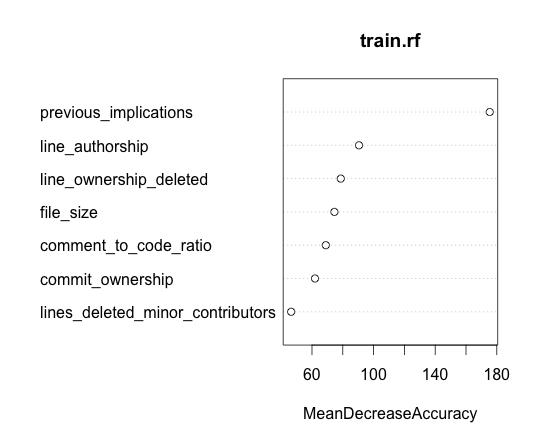
\includegraphics[width=0.45\textwidth]{images/lucene_importance_2.png}
    \caption{Importance of variables for Lucene-Solr}
    \label{fig:importance_var_lucene}
\end{figure}


%  \ref{fig:importance_var_mahout} \ref{fig:importance_var_camel} \ref{fig:importance_var_maven} \ref{fig:importance_var_zookeeper}
% \begin{figure}
%     \centering
%     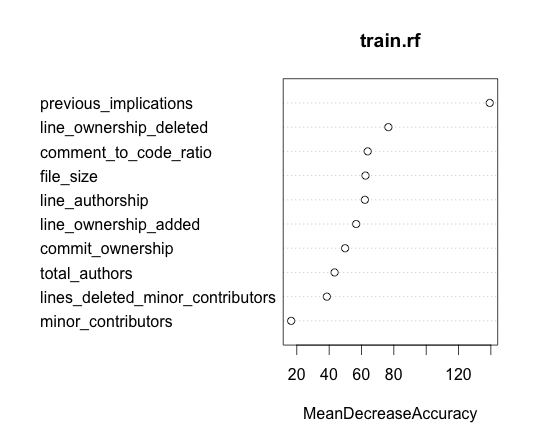
\includegraphics[width=0.45\textwidth]{images/mahout_importance_2.png}
%     \caption{Importance of variables for Mahout}
%     \label{fig:importance_var_mahout}
% \end{figure}

% \begin{figure}
%     \centering
%     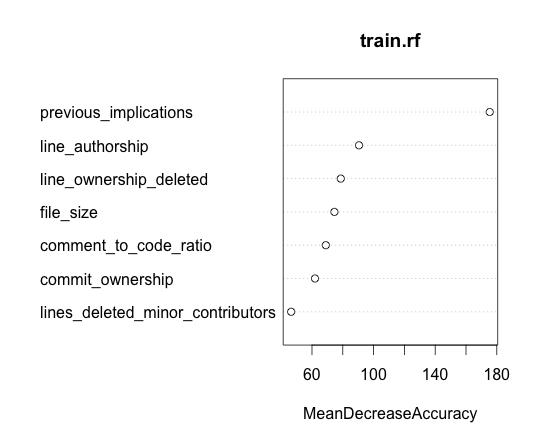
\includegraphics[width=0.45\textwidth]{images/camel_importance_2.png}
%     \caption{Importance of variables for Camel}
%     \label{fig:importance_var_camel}
% \end{figure}

% \begin{figure}
%     \centering
%     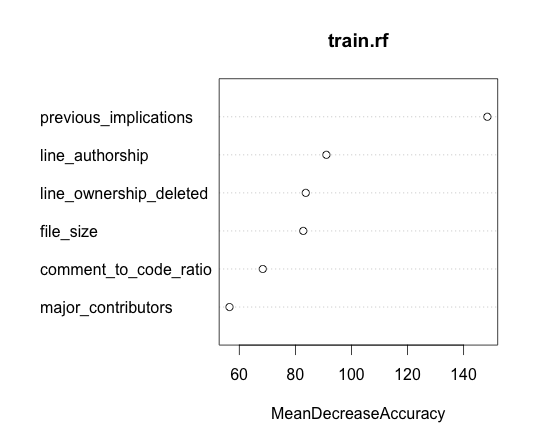
\includegraphics[width=0.45\textwidth]{images/maven_importance_2.png}
%     \caption{Importance of variables for Maven}
%     \label{fig:importance_var_maven}
% \end{figure}

% \begin{figure}
%     \centering
%     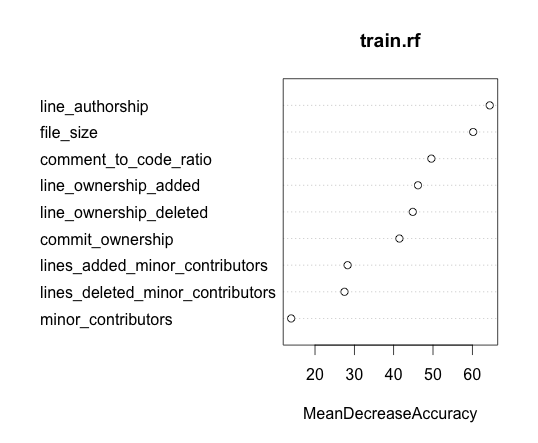
\includegraphics[width=0.45\textwidth]{images/zookeeper_importance_2.png}
%     \caption{Importance of variables for Zookeeper}
%     \label{fig:importance_var_zookeeper}
% \end{figure}

\begin{figure}[ht]
    \centering
    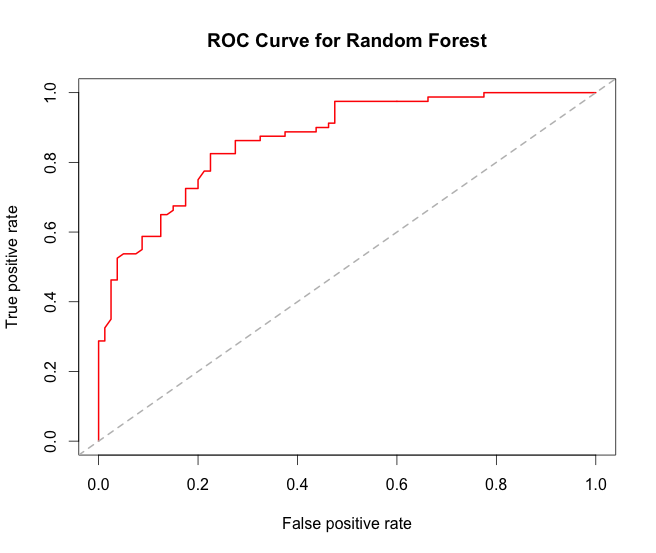
\includegraphics[width=0.45\textwidth]{images/ROC_lucene_05_all.png}
    \caption{ROC curve resulting from experiment 1 on Lucene-Solr, considering all the metrics.}
    \label{fig:roc_lucene}
\end{figure}


\subsection{Experiment 2: Logistic regression}

\subsubsection{Experiment design}

In the previous experiment we used Random Forest to determine the performance of different granularities. In this experiment we will take it a step further by taking a look at the individual metrics to see how statistically significant they are. The goal is to determine which metrics are significant, checking also if the significance changes depending on the threshold, and to determine if there is a common group of metrics that is significant for all the selected study subjects.

We determine the statistically significant metrics by running Logistic Regression on the dataset without feature selection, since this technique automatically detects which ones are not linearly dependent with each other. Logistic regression is a good choice in this case: this because it automatically computes the significance of every variable in terms of p-value.


\begin{table}[ht]
\centering
\caption{Logistic Regression outcomes explanation.}
\label{tab:significant_sym}
\begin{tabular}{cc}
\hline
Pr(>|z|) & Symbol \\
\hline
0       & $\ast\ast\ast$      \\
0.001   & $\ast\ast$          \\
0.01    & $\ast$              \\
0.05    & .                   \\
0.1     &  \\
NA      & NA\\
\hline
\end{tabular}
\end{table}

\subsubsection{Results}

Table~\ref{tab:significant_sym} shows how to interpret the results of the Logistic Regression:  NA means that the metric is considered linearly dependent with another one and because of that it is not taken into consideration. Table~\ref{tab:logistic_regression5} summarizes the results of the significance of the different metrics for the 5\% threshold.

The classic metrics are, as expected, highly significant. It can be noted that the total contributors and line authorship are also highly significant for all the projects, while the rest of the ownership metrics significance values vary a lot, meaning they are probably more project dependent. Despite that, for every project it is possible to see that at least five of these ownership metrics are statistically significant (considering a 0.05 significance level).

Table \ref{tab:experiment2_threshold} shows the influence that changing the threshold has on the significance. It can be seen there is no clear improvement in significance for the metrics, meaning that when the threshold changes the change in the significance of the metrics is not relevant: while some of them become more significant, others result to be less important. For example, when considering a 10\% threshold, \textit{lines\_added\_major\_contributors} becomes more significant for Lucene-Solr but also less significant for Mahout, in comparison to the 5\% threshold scenario. For other threshold values the results are similar.


\begin{table*}[ht]
\centering
\caption{Results of logistic regression with the metrics with a 5\% threshold, see Table~\ref{tab:significant_sym} for the interpretation.}
\label{tab:logistic_regression5}
\begin{tabular}{|c|c|c|c|c|c|}
\hline
\textbf{Metrics}                 & \textbf{Lucene-Solr} & \textbf{Camel} & \textbf{Mahout} & \textbf{Maven}  & \textbf{Zookeeper} \\ \hline
file size                        & \textbf{$\ast\ast\ast$}         & \textbf{$\ast\ast\ast$}   & \textbf{$\ast\ast\ast$}    & \textbf{$\ast\ast\ast$}    &                    \\
previous implications            & \textbf{$\ast\ast\ast$}         & \textbf{$\ast\ast\ast$}   & \textbf{$\ast\ast\ast$}    & \textbf{$\ast\ast\ast$}    & \textbf{$\ast\ast\ast$}       \\
comment to code ratio            & \textbf{.}           & \textbf{$\ast\ast\ast$}   & \textbf{$\ast\ast\ast$}    & \textbf{$\ast\ast\ast$}    & \textbf{$\ast\ast\ast$}       \\
\hline
commit ownership                 &                      & \textbf{$\ast\ast\ast$}   & \textbf{$\ast$}      & \textbf{$\ast\ast\ast$}    & \textbf{.}         \\
minor contributors               & NA                   & NA             & \textbf{$\ast\ast$}     & NA              & NA                 \\
major contributors               & \textbf{$\ast\ast\ast$}         & \textbf{$\ast\ast\ast$}   & NA              & \textbf{$\ast\ast\ast$}    & \textbf{$\ast\ast\ast$}       \\
total contributors & \textbf{$\ast\ast\ast$} & \textbf{$\ast\ast\ast$} & \textbf{$\ast\ast\ast$} & \textbf{$\ast\ast\ast$} & \textbf{$\ast\ast\ast$} \\\hline
total authors                    & \textbf{$\ast\ast\ast$}         & \textbf{}      & \textbf{}       & \textbf{}       & \textbf{$\ast\ast\ast$}       \\
line authorship                  & \textbf{$\ast\ast\ast$}         & \textbf{$\ast\ast\ast$}   & \textbf{$\ast\ast\ast$}    & \textbf{$\ast\ast\ast$}    & \textbf{$\ast\ast\ast$}       \\ \hline
line ownership added             & \textbf{}            & \textbf{$\ast\ast\ast$}   & \textbf{$\ast\ast\ast$}    & \textbf{$\ast\ast\ast$}    & \textbf{.}         \\
lines added minor contributors   & \textbf{}            & NA             & \textbf{}       & NA              & NA                 \\
lines added major contributors   & \textbf{}            & \textbf{$\ast\ast$}    & \textbf{.}      & \textbf{}       & \textbf{$\ast\ast$}        \\ \hline
line ownership deleted           & \textbf{.}           & \textbf{$\ast\ast\ast$}   & \textbf{$\ast\ast\ast$}    & \textbf{}       & \textbf{.}         \\
lines deleted minor contributors & NA                   & NA             &                 & NA              & NA                 \\
lines deleted major contributors & \textbf{$\ast$}           & \textbf{}      & \textbf{$\ast$}      & \textbf{$\ast\ast$}     & \textbf{}          \\ \hline
\textbf{Accuracy}                & \textbf{0.6325}      & \textbf{0.65}  & \textbf{0.6925} & \textbf{0.6425} & \textbf{0.59375}   \\ \hline
\end{tabular}
\end{table*}



\begin{table*}[ht]
\centering
\caption{Major contributors metrics with different granularities and the influence of the threshold for different projects}
\label{tab:experiment2_threshold}
\begin{tabular}{|c|c|c|c|c|c|c|}
\hline
\textbf{Threshold} & \textbf{Metrics} & \textbf{Lucene-solr} & \textbf{Camel} & \textbf{Mahout} & \textbf{Maven} & \textbf{Zookeeper} \\
\hline
\multirow{3}{*}{5\%} & major contributors & \textbf{$\ast\ast\ast$} & \textbf{$\ast\ast\ast$} & NA & \textbf{$\ast\ast\ast$} & \textbf{$\ast\ast\ast$} \\
 & lines added major contributors & \textbf{} & \textbf{$\ast\ast$} & \textbf{.} & \textbf{} & \textbf{$\ast\ast$} \\
 & lines deleted major contributors & \textbf{$\ast$} & \textbf{} & \textbf{$\ast$} & \textbf{$\ast\ast$} & \textbf{} \\
\hline
\multirow{3}{*}{10\%} & major contributors & \textbf{$\ast\ast\ast$} & \textbf{} & \textbf{} & \textbf{} & \textbf{$\ast\ast\ast$} \\
 & lines added major contributors & \textbf{$\ast\ast$} & \textbf{$\ast\ast\ast$} & \textbf{} & \textbf{$\ast\ast$} & \textbf{$\ast\ast\ast$} \\
 & lines deleted major contributors & \textbf{} & \textbf{} & \textbf{} & \textbf{$\ast\ast\ast$} & \textbf{} \\
\hline
\multirow{3}{*}{20\%} & major contributors & \textbf{$\ast\ast\ast$} & \textbf{$\ast\ast$} & \textbf{$\ast\ast$} & \textbf{$\ast\ast\ast$} & \textbf{.} \\
 & lines added major contributors & \textbf{$\ast\ast\ast$} & \textbf{} & \textbf{.} & \textbf{} & \textbf{} \\
 & lines deleted major contributors & \textbf{} & \textbf{} & \textbf{$\ast\ast\ast$} & \textbf{$\ast\ast\ast$} & \textbf{} \\
\hline
\multirow{3}{*}{30\%} & major contributors & \textbf{$\ast\ast\ast$} & \textbf{} & \textbf{$\ast$} & \textbf{} & \textbf{} \\
 & lines added major contributors & \textbf{$\ast\ast\ast$} & \textbf{$\ast\ast\ast$} & \textbf{$\ast\ast$} & \textbf{} & \textbf{} \\
 & lines deleted major contributors & \textbf{} & \textbf{} & \textbf{$\ast\ast\ast$} & \textbf{$\ast\ast\ast$} & \textbf{} \\
\hline
\multirow{3}{*}{40\%} & major contributors & \textbf{$\ast\ast\ast$} & \textbf{} & \textbf{$\ast\ast$} & \textbf{$\ast$} & \textbf{} \\
 & lines added major contributors & \textbf{$\ast\ast\ast$} & \textbf{$\ast\ast\ast$} & \textbf{$\ast\ast$} & \textbf{} & \textbf{.} \\
 & lines deleted major contributors & \textbf{} & \textbf{} & \textbf{$\ast$} & \textbf{$\ast\ast\ast$} & \textbf{}\\
 \hline
\end{tabular}
\end{table*}




\subsection{Experiment 3: Minor-major thresholds}

\subsubsection{Experiment design}

Research question 2b has to do with the threshold used to distinguish minor and major contributors and with how much does it influence the performance of the classifier. The goal of the experiment is to determine the effect of the different thresholds that we selected to use: \texttt{0.05}, \texttt{0.10}, \texttt{0.20}, \texttt{0.30}, and \texttt{0.40}.

As said in Section~\ref{sec:metrics}, for every project we computed a metrics dataset for each one of the thresholds. In this experiment we use again the Random Forest technique to build a classifier for every threshold and every project, considering only the metrics that depend on the threshold, so all the ones that measure minor and major contributors (see Table~\ref{tab:metrics}). This results in 25 classifiers.

The performance of every classifier is measured using 10-folds cross-validation and the OOB error: since we used only features that depend from the threshold, the difference between these resulting models is only related to its variation.

To determine if the 5 groups of OOB errors, corresponding to different thresholds, differ in a statistically significant way we apply an \textit{ANOVA} test, which will tell if the outcomes are statistically significant. Based on the output p-values we can determine if some thresholds are statistically better than other ones for some of the projects.


\subsubsection{Results}

In Table \ref{tab:resultexp2} shows the out-of-bag error for the different projects and thresholds. It can be noticed that changing the threshold doesn't give a clear increase in performance in any case. The ANOVA test shows that there is no significant outcome: all p-values are above 0.05, meaning that major-minor threshold doesn't have any significant impact on the performance.


\begin{table*}[ht]
\centering
\caption{Average performance of minor-major threshold dependent metrics}
\label{tab:resultexp2}
\begin{tabular}{|c|c|c|c|c|c|}
\hline
\textbf{Projects} & \textbf{OOB (0.05)} & \textbf{OOB (0.10)} & \textbf{OOB (0.20)} & \textbf{OOB (0.30)} & \textbf{OOB (0.40)} \\
\hline
Lucene-Solr & 44.60\% & 43.35\% & 43.60\% & 44.99\% & 46.17\% \\
Camel & 39.15\% & 37.75\% & 39.14\% & 40.26\% & 41.23\% \\
Mahout & 41.37\% & 39.89\% & 39.67\% & 43.63\% & 42.83\% \\
Maven & 38.25\% & 38.89\% & 36.66\% & 40.81\% & 42.00\% \\
Zookeeper & 33.44\% & 33.72\% & 34.82\% & 36.93\% & 34.73\% \\
\hline
\end{tabular}
\end{table*}


\subsection{Summary of results}


\textbf{RQ1,2}: Based on the results of the experiments we can say that ownership metrics are an indication for the presence of implicated code. Over the 5 projects we got an average classifier OOB of 22\% with a significant improvement over the one that uses only classic metrics (22\%).

\textbf{RQ2a}: The level of granularity used to compute the ownership metrics is important: our results show that line-based metrics give a significant improvement and are on average 15\% more effective than the commit-based ones. The authorship can also be considered a line-based ownership metric; it gives even a better improvement and it is statistically significant for all the projects. %When looking at the significance of metrics we can see that commit and line ownership added/deleted are significant for most projects, but also seem to be different per project. Line authorship is the only metric that is highly significant for all the projects.

\textbf{RQ2b}: For what concerns the threshold used to distinguish minor and major contributors, the results show that its value doesn't influence the classifier accuracy in a statistically significant way; this is due to the fact that the metrics that depend on the threshold are in general not so effective in this setup.

\subsection{Discussion}
%PAST RESULTS (FROM OTHER PAPERS):
% Bird et al.:
%   - own. metrics are effective
%   - most effective: (1) Minor (2) Ownership

% Focault et al.
%   - Not effective

% Greiler et al.:
%   - own. metrics are effective
%   - most effective: (1) Total (2) Ownership
%   - Minor = least important

% Rahman et al.
%   - Authorship is effective for OSS also, almost always (C language)
%   - both the metrics
%
% We interpret the results on the base of these:
The obtained results show that our work contributes to the research in this field, confirming some past outcomes and contradicting some others.
Bird et. al~\cite{bird:original} and Greiler et al.~\cite{Greiler:replication} showed that ownership metrics are indicative for software quality in Microsoft projects while Foucault et al.~\cite{Foucault:oss} showed the opposite regarding OSS projects. Our results confirm the fact that the effect of code ownership on software quality is highly project dependant, but we can consider ownership metrics indicative for software quality also for OSS projects, since for each one of our case studies three or more of them are significant for the classification (see Table~\ref{tab:logistic_regression5}) and considering them improves a classic code metrics model in a significant way (see Table~\ref{tab:sum_experiment_1_results}). Our result are in contrast with the ones from Focault et al.~\cite{Foucault:oss}, and the reasons could be that: (1) we try to classify defective files instead of correlate the metrics with the number of defects; (2) we consider also ownership at a line-based granularity; (3) we consider also memory-less ownership (authorship).

Looking at the metrics significance in Table~\ref{tab:logistic_regression5} we can see that \textit{total contributors} and \textit{line authorship} are the only non-classic metrics that are always significant: this confirms the results from Greiler et al.~\cite{Greiler:replication} and Rahman et al. respectively. This outcome makes sense, since the two mentioned studies tried to distinguish defective and non-defective artifacts (i.e. Microsoft source files and C language implicated code chunks) with approaches similar to our (i.e. classification). \textit{Commit ownership} was also shown to be important by Bird et al.~\cite{bird:original} and Greiler et al.~\cite{Greiler:replication}, and for us the same holds in three out of five projects. Minor and major contributors are highly dependant from each other (reasonable, since they sum to the \textit{total contributors}): for every project one of them is discarded, while the other one results significant, confirming what stated by Bird et al.~\cite{bird:original}.
